%
% File emnlp2015.tex
%
% Contact: daniele.pighin@gmail.com
%%
%% Based on the style files for ACL-2015, which were, in turn,
%% Based on the style files for ACL-2014, which were, in turn,
%% Based on the style files for ACL-2013, which were, in turn,
%% Based on the style files for ACL-2012, which were, in turn,
%% based on the style files for ACL-2011, which were, in turn, 
%% based on the style files for ACL-2010, which were, in turn, 
%% based on the style files for ACL-IJCNLP-2009, which were, in turn,
%% based on the style files for EACL-2009 and IJCNLP-2008...

%% Based on the style files for EACL 2006 by 
%%e.agirre@ehu.es or Sergi.Balari@uab.es
%% and that of ACL 08 by Joakim Nivre and Noah Smith

\documentclass[11pt,a4paper]{article}
\usepackage{acl2015}
\usepackage{times}
\usepackage{url}
\usepackage{latexsym}
\usepackage{color}
\usepackage{enumitem}
\usepackage{booktabs}
\usepackage{graphicx}
\usepackage{todonotes}


%\setlength\titlebox{5cm}

% You can expand the titlebox if you need extra space
% to show all the authors. Please do not make the titlebox
% smaller than 5cm (the original size); we will check this
% in the camera-ready version and ask you to change it back.


\title{Predicting word-sense annotation agreement}

\author{First Author \\
  Affiliation / Address line 1 \\
  Affiliation / Address line 2 \\
  Affiliation / Address line 3 \\
  {\tt email@domain} \\\And
  Second Author \\
  Affiliation / Address line 1 \\
  Affiliation / Address line 2 \\
  Affiliation / Address line 3 \\
  {\tt email@domain} \\}

\date{}

\begin{document}
\maketitle
\begin{abstract}
\section{Introduction}


In this article we propose a regression method to predict systematic disagreement, namely the variation of agreement in sense-annotated examples that depends on the linguistic features of the headword and its contexts.
 In this article we tackle the estimation of the likely agreement of a sense-annotated example by means of regression. \textcolor{red}{ We observe so and so}. 
\end{abstract}

Sense-annotation tasks show less-than-perfect agreement scores. However, variation in agreement is not the result of featureless, white noise on the annotations; \newcite{krippendorff2011} defines disagreement as \textit{by chance}---caused by unavoidable inconsistencies in annotator behavior---and \textit{systematic}---caused by properties of the data being annotated.

If we can identify linguistic properties that can predict whether an example has a low or high agreement, then we can claim that some of the agreement variation in the data is systematic, and is a result of the interplay between the linguistic properties of the examples and the characteristics of the sense inventory.



\newcite{Artstein2008} provide interpretation of Kripperdorff's $\alpha$ coefficient to describe the reliability of a whole annotation task, and the way that observed agreement ($A_o$) is calculated for each example. Strictly speaking, the value of $\alpha$ only provides an indication of the replicability of an annotation task, but we propose that the difficulty of annotating a particular example will influence its local observed agreement. Thus, easy examples will have a high $A_o$, that will drop as difficulty increases. 


%The goal of this experiment is to measure how much of the disagreement in the annotations is caused by linguistic properties of the examples and is thus systematic. More specifically, we intend to interpret the $R^2$ determination coefficient of a regression model on the linguistic features.1



Identifying low-agreement examples by their linguistic features would help characterize contexts that make words difficult to annotate. Detecting the potential agreement examples has a immediate application for data collection, as a way of estimating the proportion of examples of each difficulty level that one wants to sample. Moreover, a model of (dis)agreement can help interpret the mispredictions of a word-sense disambiguation system (a la XXX etc al) without requiring the data to be multiply annotated. 

$A_o$ is a continuous-valued variable and we tackle its prediction as regression (Section \ref{sec:reg}). We also experiment with a discretized version of observed agreement into low, mid and high agreement, which is predicted using classification (Section \ref{sec:class}).  

\paragraph{Contributions} This article provides, to the best of our knowledge, the first attempt to predict instance-wise agreement from the linguistic features of the context.
\section{Related work}
In their seminal study, \newcite{Yarowsky2002} examine on the relation between agreement variation and predictive power of word-sense disambiguation systems, which is later expanded by \newcite{Lopez2015}.
\newcite{Tomuro2001} uses the disagreement between annotators of two English sense-annotated corpora to provide insights on the relations between synsets, and more recent studies \cite{Plank2014,Jurgens2013,Jurgens2014} have empirically tackled the issue of inter-annotator disagreement as a phenomenon that is potentially informative for natural language processing, while others advocate for models of annotator behavior \cite{Passonneau2014,Cohn2013}. 

\section{Data}
\subsection{Datasets}

We conduct our study on sense-annotated datasets, keeping only the examples with at least than two annotations per item. Sometimes a whole dataset is multiply annotated. In the datasets with two annotators and one adjudicator, we disregard adjudications because they potentially have a bias that is different from the the annotators'.\\
\noindent\textsc{mascc} The English crowdsourced word-sense corpus from \newcite{Passenau2010}.\\
\textsc{masce*} The expert annotations for a series of English lexical-sample words from \newcite{Passonneau2012}, with several annotation rounds. We include the second, third and fourth round of annotation in our experiments. We evaluate on the whole dataset (\textsc{mascew}) pooling all the rounds together, as well as on each round independently, namely \textsc{masce2}, \textsc{masce3} and \textsc{masce4}.\\
\textsc{fntw} The English Twitter FrameNet data of \newcite{Sogaard2015}. We treat the frame-name layer as a word-sense layer, and disregard the arguments.\\
\textsc{ensst} The English Twitter supersense-annotated data of \newcite{Johannsen2014}.\\
\textsc{eusc} The Basque SemCor \cite{Agirre2006}.\\
\textsc{dasst} The Danish supersense data of \cite{MartinezAlonso2015}.\\
Table \ref{tab:data} provides the characteristics of the dataset. The annotation task can be lexical-sample (ls) or all-words (aw), the number of instances is different from the number of sentences for all-words annotation. The type of annotators can be expert (ex) or crowdsourced (cs). The $\alpha$ scores can differ from those reported in the datasets' documentation given our example-selection criteria. The last two columns describe the target variables of observed agreement ($A_o$) and the proportion of low-, mid- and high-agreement instances, cf. \ref{sec:targetvars} for details.

\begin{table*}[Ht!]

\begin{center}
  \begin{tabular}{llllrrrcccc}
  \toprule 

Dataset& lang & inventory & task & sent & inst & ann & type & $\alpha$ & $A_o\pm\sigma$ & /H/L/M\\ 
\midrule 

\textsc{mascc} & English & synset & ls & 44.6k & 44.6k & 13-25 & cs & .40 & .14 $\pm$ .24 & 25/44/31\\
\textsc{mascew} & English & synset & ls & 2.6k & 2.6k & 2-6 & ex & .48 & .07 $\pm$ .35 & 24/21/55\\
---\textsc{masce2} & English & synset & ls & 1.5k & 1.5k & 5-6 & ex & .51 & .41 $\pm$ .3 & 21/36/43\\
---\textsc{masce3} & English & synset & ls & 500 & 500 & 3 & ex & .69 & .80 $\pm$ .33 & 28/00/72\\
---\textsc{macse4} & English & synset & ls & 618 & 618 & 2 & ex & .63 & .73 $\pm$ .44 & 27/00/73\\
\textsc{ensst} & English & supersense & aw & 39 & 326 & 3 & ex & .67 & .69 $\pm$ .36 & 45/00/55\\
\textsc{fntw} & English & frame & aw & 236 & 958 & 3 & ex & .82 & .82 $\pm$ .31 & .26/00/74\\

\textsc{eusc} & Basque & synset & ls & 20.6k & 20.6k & 2 & ex & .76 & .76 $\pm$ .43 & 240/0/76\\
\textsc{dasst} & Danish & supersense & aw & 1.2k & 9.5k & 2 & ex & .65 & .67 $\pm$ .47 & 33/00/67\\


\bottomrule

  \end{tabular}  
\end{center}
\caption{Dataset characteristics \label{tab:data} in terms of language, sense inventory, type of annotation task, number of sentences, number of isntances, number of annotators, type of annotators, Krippendorff's $\alpha$, observed agreement and percentage of LOW/MID/HIGH agreement examples.}
\end{table*} 

\subsection{Features}
We define an \textit{instance} as a sentence with a target word for annotation. If a sentence has $n$ annotated target words, it yields $n$ instances. For each instance, we calculate the following features for a word $w$ and its syntactic parent $p$ in a sentence $s$, organized in feature groups.\\ 
\noindent\textbf{Frequency(2)} We calculate the frequency of $w$ and $p$, scaling the frequencies by $log(rank(x)+1)^{-1}$.\\
\textbf{ Morphology (5)} We consider the part-of-speech tag (POS) of $w$, of $p$,and the POS-bigram at the left and at the right of $w$. In order to incorporate information on inflectional complexity, we calculate which proportion of the stem of $w$ is covered by $w$, e.g. the occurrences of `jumping' constitute 22\% of the occurrences of the stem `jump'. \\
\textbf{Syntax (5)} We calculate the number of dependents of $w$ and $p$, and a bag of words for the labels of the dependents of $w$ and $p$. We also include the distance from $w$ to the root node, and the linear distance between $w$ and $p$.\\
\textbf{ Context  (5)} We calculate the amount length of $s$ in tokens, the proportion of $w$ made up of content words, and a bag of words of the context of $w$, i.e. all the words of $s$ except $w$. In order to capture the specificity of the context, we calculate the maximum and the sum of the entence-wise idf of each stem in $s$ \\
\textbf{Sense inventory (2)} We calculate the amount of possible senses for $w$, including an additional sense when $w$ could be discarded from the annotation---like the tag `O' for supersenses--- or the right synset was not present in WordNet. We also calculate the sense entropy for each word following \newcite{Yarowsky2002}. 

Note that the word identity of $w$ and $p$ are not included in the features to keep the models more general. We use TreeTagger (CITE) for part-of-speech tagging and TurboParser (CITE) for dependency parsing. All tagging and parsing models are trained on the Universal Dependencies v1.1 \footnote{\url{https://lindat.mff.cuni.cz/repository/xmlui/handle/11234/LRT-1478}}, which allows cross-language comparison of features. We estimate frequencies on 100M-word web-crawled and Wikipedia corpora for English and Danish, and on 13M newswire for Basque.

\subsection{Target variable}
\paragraph*{Regression} Instance-wise observed agreement ($A_o$) is the target variable for the regression experiments. We calculate  the $A_o$ for each example by calculating the pairwise matches in the annotation and dividing over the amount of pairwise combinations of annotation. 
Note that the $\alpha$ coefficient is an aggregate measure that is obtained dataset-wise, and $A_o$ is the only agreement measure available for each individual example.
\paragraph*{Classification} Agreement level is the target variable for the classification experiments, where we discretize $A_o$ into the three classes, namely LOW , MID and HIGH. We set the threshold for LOW at $Ao \le \frac{1}{3}$, for HIGH at $Ao \ge \frac{2}{3}$, and intermediate values receive the label MID.


\section{Experimental setup}
We use the sklearn\footnote{\url{http://scikit-learn.org/}} implementation for all learning algorithms, and train and test on 10-fold cross validation.

\paragraph*{Regression} We use L2-regularized linear regression. The output of the regression is sigmoid-transformed to keep the values in the range $[0,1]$. The baselines for regression are \textsc{mean}, where all instances receive the mean $A_o$ of the dataset, and  \textsc{median}, where the assigned value is the median $A_o$. 

\paragraph*{Classification} We use a maximum entropy classifier. The baselines for classification are \textsc{mfc}, where all instances receive most frequent class, and the two random baselines \textsc{stra}, where the assigned values are randomly selected via stratified sampling from the distribution of classes in the dataset, and \textsc{uni} where random values are assigned from the uniform distribution of the three possible classes . 

\subsection{Results}
\subsubsection{Regression}

Table \ref{tab:regagr_results} shows the results for regression.


\begin{table}[Ht!]

\begin{center}
  \begin{tabular}{lc|cc}
 \toprule
 & \textsc{Regression} & \textsc{mean} & \textsc{median} \\
 \midrule
 \textsc{mascc} & 0.19 & 0.21 & 0.21 \\
 \textsc{mascew} & 0.31 & 0.32 & 0.37 \\
---\textsc{masce2} & \textbf{0.27} & 0.26 & 0.25 \\
---\textsc{masce3} &\textbf{ 0.36} & 0.29 & 0.20 \\
---\textsc{masce4} & \textbf{0.46} & 0.40 & 0.27 \\
\textsc{ensst} & \textbf{0.43} & 0.35 & 0.31 \\
\textsc{fntw} & \textbf{0.27} & 0.26 & 0.18 \\

\textsc{eusc} & 0.35 & 0.37 & 0.24 \\
\textsc{dasst} & 0.42 & 0.44 & 0.33 \\

\bottomrule

  \end{tabular}  
\end{center}
\caption{Agreement prediction as regression compared against mean and median $A_o$. Datasets where the system outperforms the hardest baseline are marked in bold. \label{tab:regagr_results}}
\end{table} 

We will consider the proportion of explained variance of the regression model described by the coefficient of determination $R^2$ to be the amount of disagreement our system can give account for, and is thus systematic. 


For positive values of $R^2$, we can claim that there is at least that much proportion of the disagreement that can be explained by the features and is thus systematic. A smoother target variable is easier to fit. Fewer annotators per item yield more jagged distributions of $A_o$, with fewer different intermediate values. The higher the amount of annotators, the better the resolution of the target variable. 


$R^2$ does not strictly say how much agreement is systematic, but how much of the agreement variation within a dataset can be explained by the features. Regression models for datasets that have very low or very high agreement and little variation cannot be so easily fit, because regression fitting benefits from smoothness in the dependent variable, while (discriminative) classification relies on the complementary notion of linear separability. In other words, some datasets lend themselves better to regression than others.


\subsubsection{Classification}
Table \ref{tab:classresults} shows the results for classification.


\begin{table}[Ht!]

\begin{center}
  \begin{tabular}{lc|ccc}
 \toprule
 & \textsc{MaxEnt} & \textsc{MFC} & \textsc{stra} & \textsc{uni} \\
 \midrule
 \textsc{mascc} & \textbf{0.45} & 0.27 & 0.35 & 0.37\\ 

 \textsc{mascew} & \textbf{0.48} & 0.39 & 0.39 & 0.35\\ 
---\textsc{masce2} & \textbf{0.39} & 0.25 & 0.34 & 0.33\\ 
---\textsc{masce3} & \textbf{0.62} & 0.60 & 0.57 & 0.53\\ 
---\textsc{masce4} & \textbf{0.63} & 0.62 & 0.62 & 0.55\\ 
\textsc{ensst} & 0.50 & 0.39 & 0.51 & 0.49\\ 
\textsc{fntw} & \textbf{0.71} & 0.63 & 0.61 & 0.51\\ 

\textsc{eusc}  & \textbf{0.68} & 0.65 & 0.63 & 0.54 \\
\textsc{dasst} & \textbf{0.60} & 0.53 & 0.55 & 0.53\\ 

\bottomrule

  \end{tabular}  
\end{center}
\caption{Agreement prediction as classification compared against the most-frequent, stratified and uniform baseline. Datasets where the system outperforms the hardest baseline are marked in bold. \label{tab:classresults}.}
\end{table} 

The two Twitter datasets (XXXX and XXXX) show very different behavior. The framenet dataset has a very large  amount of instances where the amount of possible senses is very low, while the amount of possible senses is always large (XXX) for the Supersense data. \textcolor{red}{The preannotation of the framenet data makes it more streamlined and provides artificial agreement, while the open-guideline free method for the SST data is more exposed to the domain problems of Twitter. I think a lot of the bad performance on TWitter has to do with the badness of the automatically generated features, WHILE for Framenet the sense-inventory features might be the most relevant}


%\begin{figure*}[htt]
%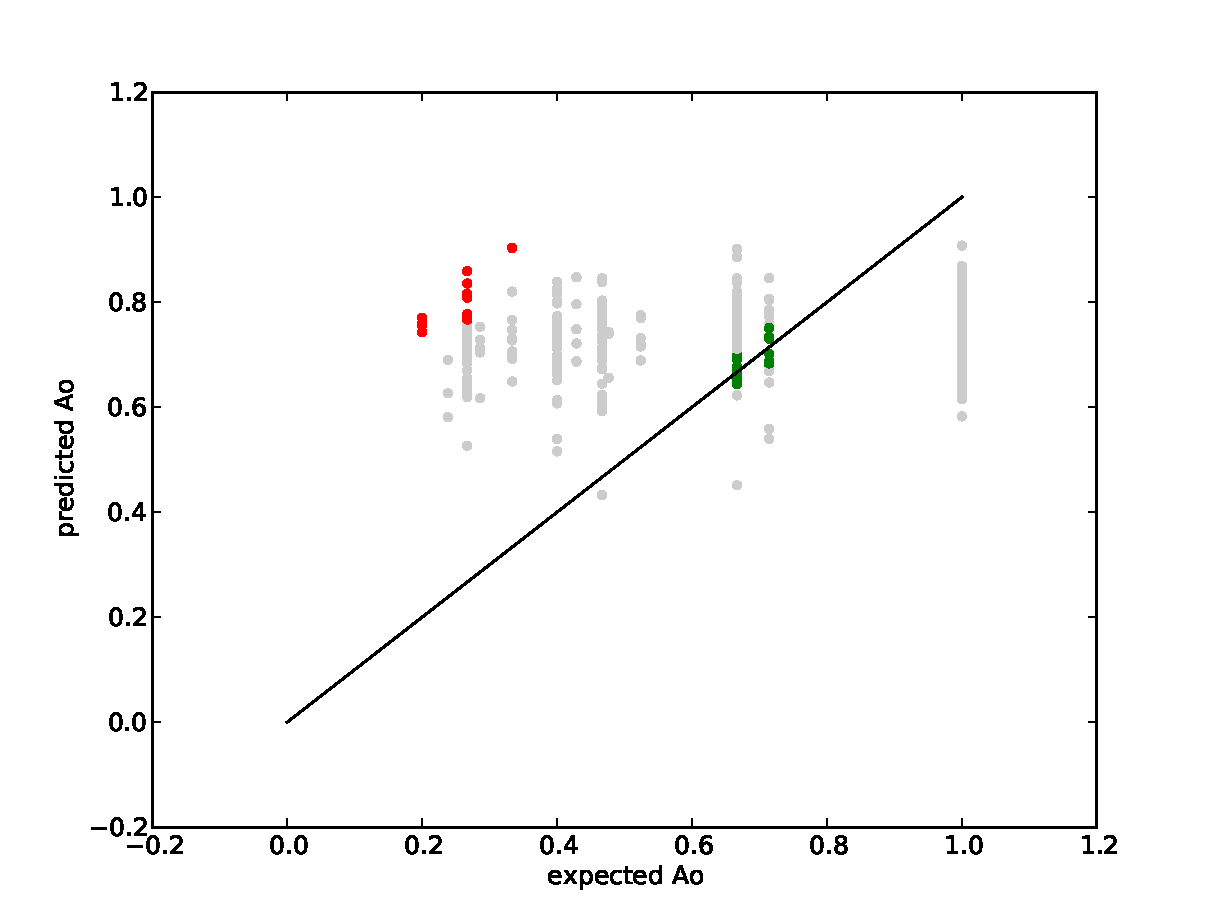
\includegraphics[scale=0.25]{scatterdraft.pdf}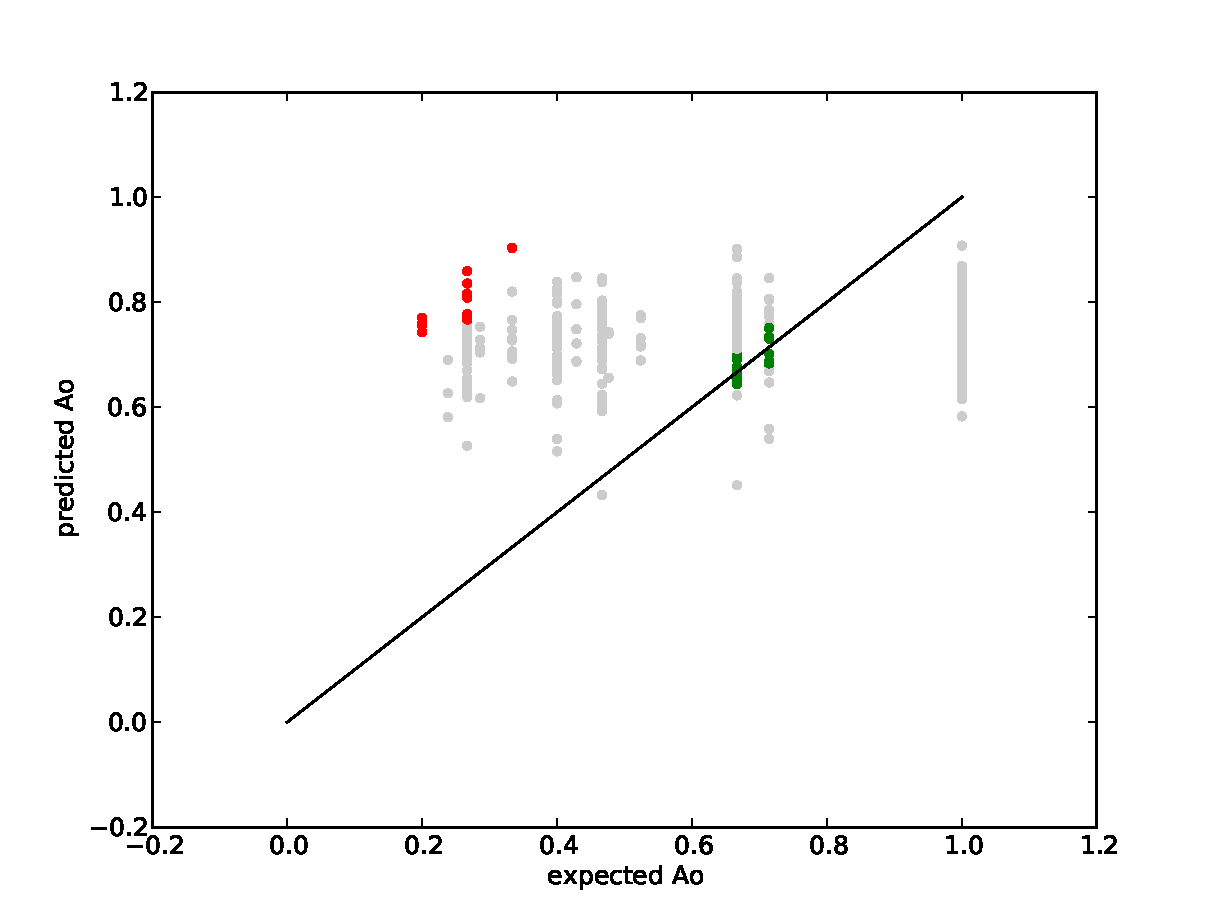
\includegraphics[scale=0.25]{scatterdraft.pdf}
%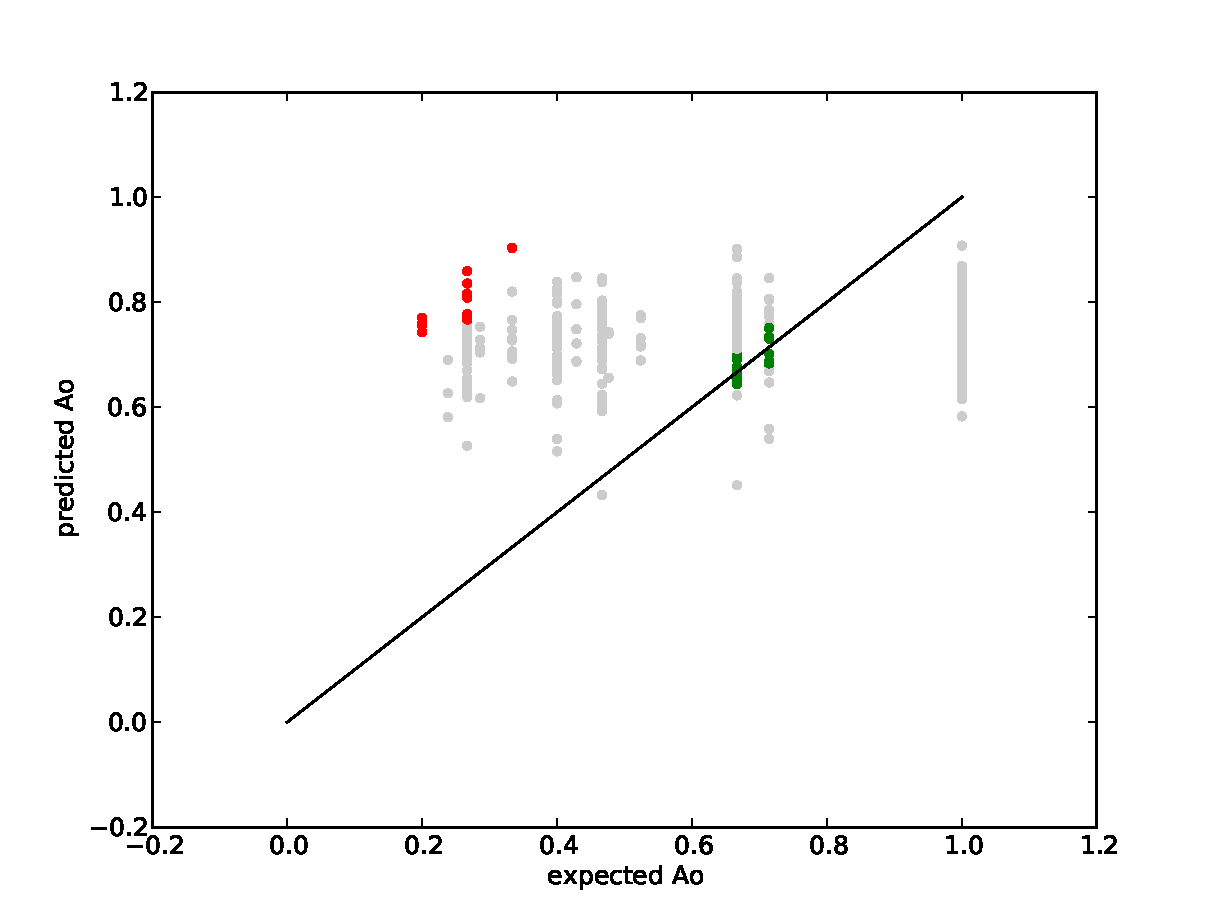
\includegraphics[scale=0.25]{scatterdraft.pdf}
%
%\caption{ \label{fig:reglit_dklocorg}\textcolor{red}{Comparative scatterplots for some datasets}}    
%\end{figure*}

% include your own bib file like this:
%\bibliographystyle{acl}
%\bibliography{acl2015}

\subsubsection{Analysis}

\begin{figure}[htt]
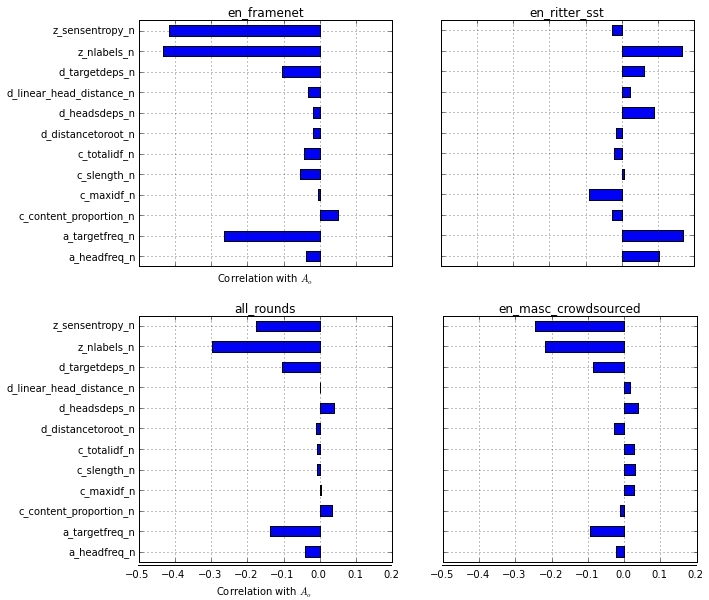
\includegraphics[scale=0.3]{corrtable.jpg}

\caption{ \label{fig:correlations}Correlation between the numeric-valued features and $A_o$ for the four English datasets}    
\end{figure}

\section{Conclusions and further work}

We have described a method to model agreement as a continuous value  the observed agreement $A_o$, and as a discrete value. We have conduct experiments on XXXX datasets, which comprise three languages, all-words vs. lexical-sample word annotations, and crowdsourced vs. expert annotations. Our findings reveal that \todo{They do reveal something right?}

 The learnability of the task is limited by the resolution of the target variable, the annotator bias (more relevant for crowdsourcing, as a result of the risk-avoiding strategy many turkers use), and the performance of the predictions for part of speech and syntactic dependencies.


\textcolor{red}{We observe that syntactic features correlate with high agreement, which implies that marked syntactic contexts help an univocal interpretation. Most negative features for agreement are lexical, which indicates that difficult or unusual words get on the way of annotator agreement. However, we have found linguistic cues that pinpoint to syntactic behavior of the headword that cause agreement to drop, because annotators interpret them in different manners. }

This system can be used as an automatic review method for sense-annotation tasks, because it identifies a proportion of systematic disagreement that can be attributed to certain linguistic features, which can lead to reviews of annotation guidelines. 


\section{Further work}
The overall conclusiveness of the study requires expanding this research to more datasets and languages, and well as further exploring the difference in annotator bias between  expert or crowdsourced annotations. Moreover, our feature repertoire does not include characteristics of the sense inventory in terms of sense relatedness like autohyponymy, depth in the sense ontology, or qualitative properties of the potential senses like whether they are abstract. Also, at this current stage, we do not include feature interactions in our models.

If the numeric prediction of agreement is desirable, it is worth considering alternative measures to $A_o$ that are more robust against singularities of the data such as the damaging effect in the pairwise comparisons of having many annotators. A possible candidate measure is annotation entropy \cite{Yarowsky2002}.

\bibliographystyle{acl}
\bibliography{biblio}

\end{document}
